\documentclass{article}

\usepackage{lmodern}
\usepackage[T1]{fontenc}
\usepackage[spanish,activeacute]{babel}
\usepackage{mathtools}
\usepackage{amsmath}
\usepackage[a5paper,margin=1in,top=15mm,bottom=15mm,landscape]{geometry} 
\usepackage{graphicx}

\graphicspath{ {./imagenes/} }
\title{\textbf{Pr\'actica 2}}
\author{\\Diego Jes\'us Romero Luque}
\date{\today}

\begin{document}
\maketitle
\pagebreak

\begin{enumerate}
    \item Consider the language over the alphabet $\{a,b\}$ that only contains the string \textit{a}.
          \begin{enumerate}
              \item Build a DFA that recognizes this language and rejects all those strings that do not belong to the language.\\
                    $M=(\{q_0,q_1,q_2\}, \{a,b\}, \delta, q_0, \{q_1\})$ with:\\
                    \begin{table}[h!]
                        \begin{tabular}{c|c|c}
                            $\delta(q,\sigma)$ & $a$   & $b$   \\
                            \hline
                            $q_0$              & $q_1$ & $q_2$ \\
                            \hline
                            $q_1$              & $q_2$ & $q_2$ \\
                            \hline
                            $q_2$              & $q_2$ & $q_2$
                        \end{tabular}
                    \end{table}

              \item Test the automaton that you have created by introducing 6 chains.
              
                    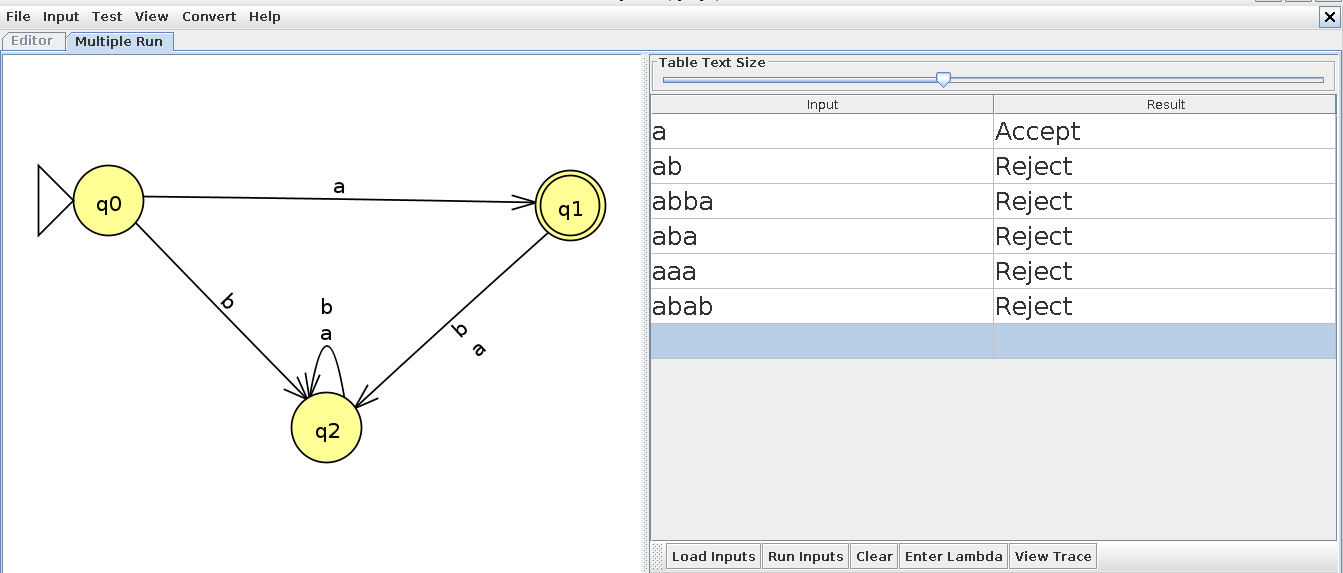
\includegraphics[scale=0.5]{Test6Chains}
          \end{enumerate}

    \item Finite automaton in Octave:
          \begin{enumerate}
              \item Open the Octave finiteautomata.m script and test it with the given example (see script help) in the GitHub repository.\\
                        $octave:12> finiteautomata("aa*bb*", "ab")$\\
                        $M = ({q0, q1, q2}, {a, b}, q0, {q2}, {(q0, a, q1), (q1, a, q1), (q1, b, q2), (q2, b, q2)})$\\
                        $w = ab$\\
                        $(q0, ab) \vdash (q1, b) \vdash (q2, \epsilon)$\\
                        $x \in L(M)$\\
                        $ans = 1$\\
              \item Specify in finiteautomata.json the automaton created in Activity 1 and test it with the script!
                    finiteautomata.json:
                    \begin{verbatim}
                  {
                      "name" : "a*",
                      "representation" : {
                        "K" : ["q0", "q1", "q2"],
                        "A" : ["a", "b"],
                        "s" : "q0",
                        "F" : ["q1"],
                        "t" : [["q0", "a", "q1"],
                               ["q0", "b", "q2"],
                               ["q1", "a", "q2"],
                               ["q1", "b", "q2"],
                               ["q2", "a", "q2"],
                               ["q2", "b", "q2"]]
                        }
                    }
              \end{verbatim}
                $octave:15> finiteautomata("a","a")$\\
                $M = ({q0, q1, q2}, {a, b}, q0, {q1}, {(q0, a, q1), (q0, b, q2), (q1, a, q2), (q1, b, q2), (q2, a, q2), (q2, b, q2)})$\\
                $w = a$\\
                $(q0, a) \vdash (q1, \epsilon)$\\
                $x \in L(M)$\\
                $ans = 1$
          \end{enumerate}

\end{enumerate}
\pagebreak



\end{document}